\documentclass[14pt]{extarticle}
\usepackage[
left=30mm,
top=20mm,
right=15mm,
bottom=20mm,
]{geometry}

\usepackage{graphicx}
\usepackage[utf8]{inputenc}
\usepackage[english, russian]{babel}
\usepackage[T1]{fontenc}
\usepackage{listings}
\usepackage{cite}
\usepackage{hyperref}
\usepackage{etoolbox}
\usepackage{indentfirst}
\usepackage{setspace}
\usepackage{tikz}
\usepackage{pgfplots}
\usepackage{float}
\restylefloat{table}
\pgfplotsset{compat=1.9}

\usepackage[linesnumbered,boxed]{algorithm2e}
\sloppy

\lstset{
	sensitive=true,
	basicstyle=\small,
	keywordstyle=\color{black},
	commentstyle=\scriptsize\rmfamily,
	keywordstyle=\ttfamily\underbar,
	identifierstyle=\ttfamily,
	basewidth={0.5em,0.5em},
	columns=fixed,
	fontadjust=true,
	literate={->}{{$\to$}}1
}

\makeatletter
%\renewcommand{\@biblabel}[1]{#1.} % Заменяем библиографию с квадратных скобок на точку:
\makeatother
\gappto\captionsrussian{\renewcommand{\contentsname}{Оглавление}}
\renewcommand\baselinestretch{1.5}
\renewcommand{\lstlistingname}{Листинг}

\begin{document}
	
	\begin{titlepage}
		\thispagestyle{empty}
		\def\baselinestretch{1.0}
		\begin{center}
			{Правительство Российской Федерации \\ \vskip 0.0em { Федеральное государственное бюджетное образовательное учреждение \\ \vskip 0.0em {высшего профессионального образования \\ \vskip 0.0em { «Санкт-Петербургский государственный университет» \\ \vskip 1.7em{\large Кафедра системного программирования \\}}}}}
			\vspace*{0.05\textheight}
			{\large Поздин Дмитрий Евгеньевич}
			
			\vskip 2em
			{\huge Оптимизированная интерпретация языка PostScript}
			
			\vskip 1em
			{\large Выпускная квалификационная работа специалиста} \\
			\vskip 2em
%			{\normalsize \raggedleft 
			{\large \raggedleft 

				Допущена к защите.\\
				Зав. кафедрой:\\
				д.ф.-м.н., проф. А.Н. Терехов
				\\[2em]
				Научный руководитель:\\
				к.ф.-м.н., доц. Д.Ю. Булычев
				\\[2em]
				Рецензент:\\
				к.ф.-м.н., доц. Д.В. Кознов
				\\[1em]
				%Неизвестно \\
				\vspace*{0.08\textheight}
				{\centering Санкт-Петербург \\ 2015}
			}
		\end{center}
	\end{titlepage}
	\begin{titlepage}
		\thispagestyle{empty}
		\def\baselinestretch{1.0}
		\begin{center}
			{SAINT-PETERSBURG STATE UNIVERSITY  \\ \vskip 0.3em{\large Chair of Software Engineering \\}}
			\vspace*{0.15\textheight}
			{\large Dmitri Pozdin}
			
			\vskip 2em
			{\huge Optimised PostScript interpretation}
			
			\vskip 1em
			{\large Graduation Thesis} \\
			\vskip 2em
			{\large \raggedleft 
				Adnitted for defence.\\
				Head of the chair:\\
				Professor  Andrey Terekhov
				\\[3em]
				Scientific supervisor:\\
				Dmitri Boulytchev
				\\[3em]
				Reviewer:\\
				Dmitry Koznov
				\\[3em]
				%Неизвестно \\
				\vspace*{0.05\textheight}
				{\centering Saint-Petersburg \\ 2015}
			}
		\end{center}
	\end{titlepage}
	
	\setcounter{page}{3}
	\tableofcontents
	%\thispagestyle{empty} 
	\pagebreak
	
	

	\section*{Введение}
	\addcontentsline{toc}{section}{Введение}
	Язык PostScript --- это  специализированный кроссплатформенный язык программирования, разработанный в начале восьмидесятых годов в компании Adobe Systems для поддержки вывода на печать документов, содержащих векторную и растровую графику. Приложения на языке PostScript представляют собой программу для построения рисунков и текстов. Основная цель создания языка заключалась в том, чтобы обеспечить аппаратно-независимую поддержку сложной цифровой графики. Язык получил широкое распространение, интерпретаторы PostScript используются в принтерах, редакторах документов (\TeX, Adobe Reader) и графических редакторах (Photoshop, Inkscape) в виде программных или аппаратных компонентов. На данный момент широко известны следующие промышленные реализации интерпретатора PostScript: GhostScript~\cite{GS-site}, Adobe PostScript~\cite{Adobe-PS-site}. 
	
	Для того, чтобы исполнять на разных устройствах PostScript-программы, для каждого из них необходим свой интерпретатор или один кроссплатформенный интерпретатор. В качестве базы для кроссплатформенного интерпретатора можно взять Java Virtual Machine, поскольку она реализована для большого числа платформ и архитектур.
	
	В лаборатории JetBrains математико-механического факультета СПбГУ был разработан интерпретатор на платформе Java для языка Postscript (далее --- интерпретатор JB). В текущий момент на основе интерпретатора ведётся разработка оконного менеджера и библиотеки примитивов для реализации графического интерфейса приложений с помощью языка PostScript. Вся работа делится на три части: оптимизированная интерпретация языка PosctScript, механизм обработки событий и реализация графических примитивов и оконного менеджера.
	
	Из-за двухуровневой модели исполнения (уровень Postscript и уровень Java) у интерпретатора JB недостаточно высокая скорость работы по сравнению с  аналогами, и поэтому существует необходимость улучшить его производительность. В процессе анализа задачи оптимизации существующего интерпретатора было выявлено два узких места. 
	
	Первой проблемой было то, что процедуры в PostScript-программах исполняются много раз, при этом каждый раз они интерпретируются заново, что существенно замедляет работу интерпретатора. Данную проблему можно решить с помощью динамической компиляции процедур в байт-код JVM.
	
	Следующей выявленной проблемой было повторное исполнение объектов-имен (англ. "name"\,~\cite{PLRM}), во время которого происходит поиск сохранённого по имени значения в стеке словарей. Для оптимизации интерпретатора было принято предположение о том, что во многих случаях объекты-имена не перезаписываются, и для улучшения скорости работы интерпретатора можно использовать кэширование имен во время компиляции процедур во избежание повторного поиска по словарям, что называется спекулятивной компиляцией.
	\pagebreak
	\section{Постановка задачи} 
	Цель данной дипломной работы заключалась в оптимизации работы интерпретатора JB для повышения скорости его работы. Для этого необходимо решить следующие задачи.
	\begin{itemize}
		\item Выполнить оптимизацию исполнения программ на языке PostScript в среде JVM посредством динамической компиляции (JIT).
		\item Выполнить оптимизацию исполнению программ на языке PostScript в среде JVM посредством спекулятивной компиляции.	
		\item Провести эксперименты по замеру производительности и проанализировать полученные результаты. 
	\end{itemize}
	
	\pagebreak
	\section{Обзор}
	В данном разделе рассмотрены особенности языка PostScript, интерпретатора GhostScript, интерпретатора JB, проекта по созданию графической библиотеки в целом и инструменты, использовавшиеся при разработке.
	\subsection{Язык Postscript}
	Данный язык является динамически типизированным, стековым языком с обратной польской нотацией. Он предназначен для отрисовки сложной векторной и растровой графики. Программы на PostScript обычно создаются другими приложениями, но при этом на PostScript  можно писать как на обычном языке программирования. 
	
	\subsubsection*{Объекты}	
	Программа на языке PostScript состоит из токенов (простейших лексических единиц), каждый из которых является объектом языка. Простые объекты хранят свое непосредственное значение, в то время как сложные --- только ссылку на него. В языке используются следующие примитивные типы: \texttt{int}, \texttt{real}, \texttt{boolean}, \texttt{name}, \texttt{operator}, \texttt{mark}. Поддерживаются также сложные типы объектов, такие как: \texttt{string}, \texttt{array}, \texttt{dictionary}, \texttt{save}. Все объекты могут быть либо литеральными (от англ. "literal"), и в этом случае объект просто кладется на стек во время исполнения, либо исполняемыми. Это свойство записано в соответствующем атрибуте объекта. 
	
	 Имена (тип \texttt{name}) --- это аналог переменных в других языках. Литеральное имя используется для записи, а исполняемое --- для вызова соответствующего значения. Поскольку в PostScript используется стратегия вычислений \texttt{вызов-по-имени} (англ. "call-by-name"), то связывание имен со значением происходит в момент исполнения это имени. Кроме того, любое имя можно переопределить в любом месте программы, в том числе и то, которое связано со стандартным оператором. 
	 
	 Массивы (тип \texttt{array}) бывают литеральными, и тогда они являются структурами данных, или исполняемыми, тогда они играют роль процедур. Процедуры --- это набор объектов, которые необходимо исполнить. В тексте программы процедуры выглядят как блок кода, ограниченный фигурными скобками.
	 
	 \subsubsection*{Архитектура}
	 В интерпретаторе языка есть четыре стека: графический стек, стек операндов, стек словарей и стек вызовов. Каждый из них отвечает за свои функции. Стек операндов хранит аргументы для операторов. Стек словарей --- это структура, которая хранит данные о всех переменных. В каждом словаре, который находится на этом стеке, имена ассоциированы со своими значениями. В графическом стеке хранятся настройки графики, например: цвет, текущий путь и др. Стек вызовов отвечает за исполнение программы, каждый его элемент является процедурой.
	 \subsubsection*{Механизм исполнения}
	 Исполнение программы на PostScript происходит "объект за объектом". Например, если очередной объект --- исполняемый массив, то он кладется на стек вызовов в качестве новой процедуры, и после этого исполняются объекты уже в этой процедуре. Таким образом, на стеке вызовов находятся прерванные процедуры, и на вершине стека --- текущая исполняемая процедура.
	 \subsubsection*{Виды операторов}
	 В PostScript существует большое количество операторов, которые находятся в одном словаре, называющимся системным. Среди операторов можно выделить несколько больших групп: арифметические, логические, для работы с стеками и разными типами объектов, для построения пути, рисования, и прочие. 
 
	 \subsection{Обзор промышленного интерпретатора Ghostscript}
	 Одной из промышленных реализаций интерпретатора PostScript является GhostScript, продукт компании Artifex Software~\cite{artifex-site}. Первая версия была выпущена в 2000 году, и новые версии выходят до сих пор. GhostScript перенесён для операционных систем Linux, Mac OS X, Unix-подобных и Windows.
	%\pagebreak 
	\subsection{Описание интерпретатора языка PostScript}
	%В лаборатории JetBrains математико-механического факультета СПбГУ был спроектирован и разработан интерпретатор языка PostScript (далее --- интерпретатор JB).
	В качестве платформы для интерпретатора JB выбрана Java. Этот выбор был обусловлен тем, что эта платформа обеспечивает  кроссплатформенность. Интерпретатор JB позволяет исполнять файлы PostScript, выводя на экран изображение, которое является результатом работы программы. Реализованы значительное подмножество языка, общая архитектура, все основные типы данных, механизм исполнения. 
	
	Проект по созданию интерпретатора делился на три основные части:
	\begin{itemize}
		\item Реализация общей поддержки времени исполнения для интерпретатора языка PostScript~\cite{runtime}.
		\item Реализация графической части интерпретатора языка PostScript~\cite{graphic}.
		\item Архитектура интерпретатора для исполнения программ на языке PostScript в JVM~\cite{architecture}.
	\end{itemize}

		
	 
	\subsection{Интерпретатор JB и GhostScript}
	Интерпретатор GhostScript рассматривался в качестве эталонного при разработке интерпретатора JB. В GhostScript реализованы все системные операторы из спецификации. Поэтому именно он использовался для проверки корректности работы операторов и построения рисунка в целом в интерпретаторе JB.
		
	
	\subsection{Описание проекта по созданию графической \\ библиотеки на основе PostScript}	
	На основе интерпретатора JB  в лаборатории JetBrains разрабатывается графическая библиотека. При этом все графические примитивы (кнопки, окна и т.д.) хранятся и отрисовываются при помощи PostScript. Оконный менеджер является интерактивным, т.е. в нем перехватываются события мыши и клавиатуры, происходит взаимодействие и перерисовка изменившихся элементов интерфейса.  Преимущество данного подхода заключается в гибкости построения графического интерфейса, при этом в разных системах интерфейс будет выглядеть одинаково. Кроме того, в оконном менеджере можно добавить свои эффекты, например, переворот окна или эффект «волны».
	
	Для обеспечения высокой производительности оконного менеджера проводится оптимизация его работы, описанная в данной дипломной работе. Сам проект разделяется на два основных направления работы: механизм обработки событий в графической библиотеке и реализация примитивов и оконного менеджера (см. рис.~\ref{project_scheme}). 
	
	\begin{figure} [h]
			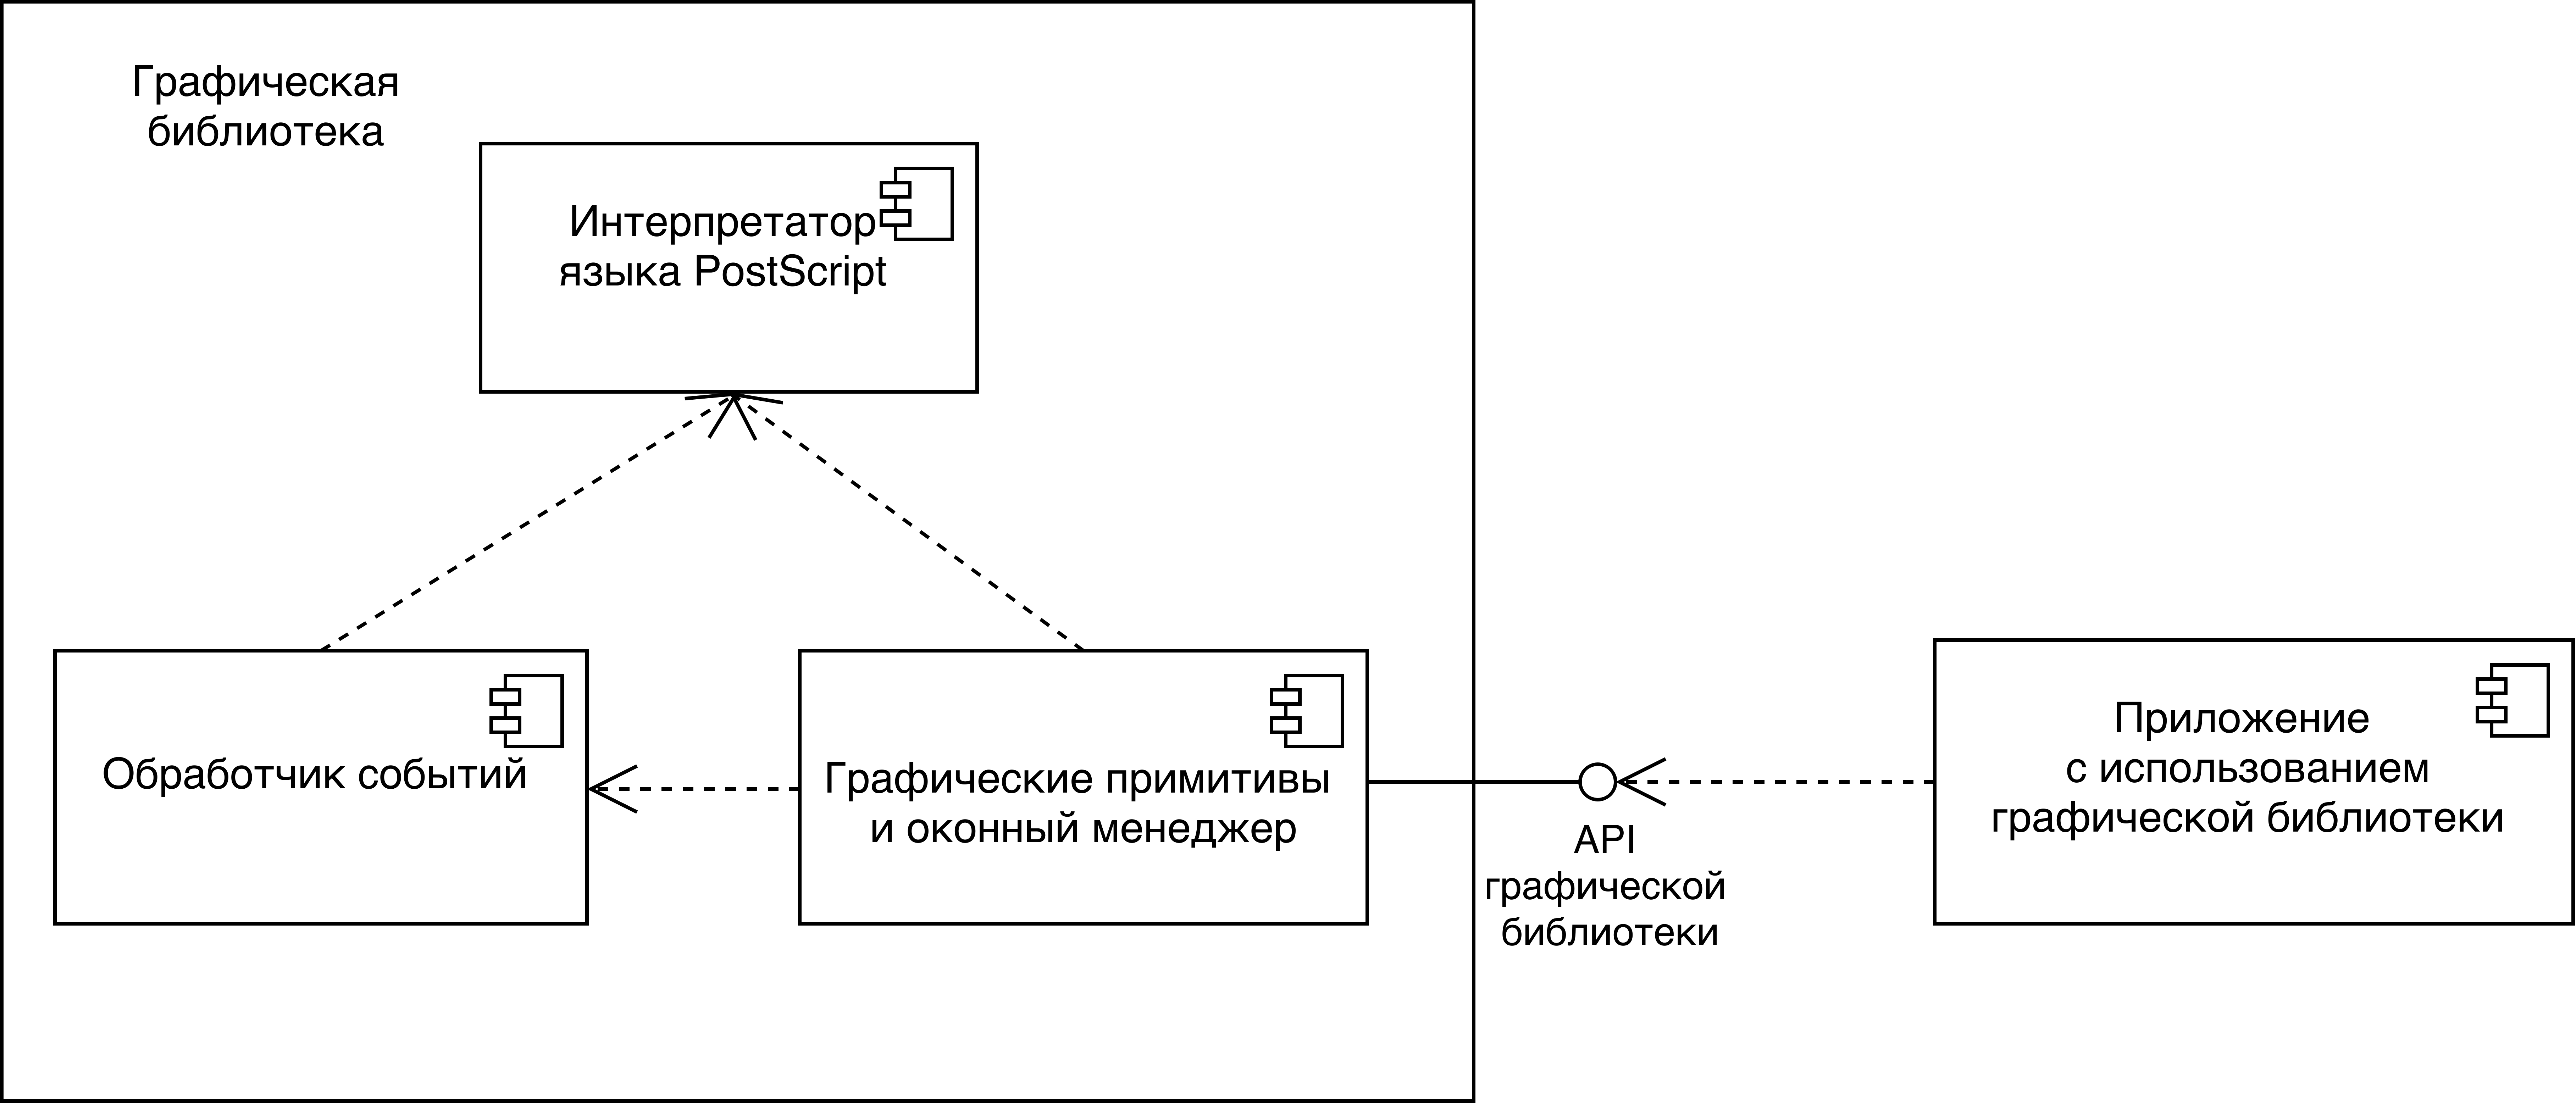
\includegraphics[height=200pt]{Project_scheme.png}
			\caption{Схема проекта}\label{project_scheme}
	\end{figure}

	\subsubsection*{Контексты и многопоточность}
	В первоначальной реализации интерпретатора JB все основные компоненты: все стеки, локальная память и интерфейс к ним --- находились в главном классе \texttt{Runtime}, в котором был реализован шаблон ООП «одиночка» (англ. "singleton")~\cite{patterns}, и из любого места интерпретатора можно было к нему обратиться. Данная схема подходила только для однопоточного исполнения программ на PostScript. Спецификация языка вообще не предусматривает многопоточность, которая необходима для реализации графических эффектов в графической библиотеке.
		
	Таким образом, возникла необходимость расширить язык и оптимизировать его для многопоточного исполнения. Каждый поток должен иметь свой набор стеков и оперировать ими. Теперь каждый поток хранит свой контекст исполнения, в котором  содержатся стеки, интерфейсы к ним и другие данные, необходимые потоку. В классе \texttt{Runtime}  остались только локальная память и механизм управления потоками. (см. рис. ~\ref{UML_runtime_contexts}) 
		
	При такой многопоточной схеме в момент выполнения  каждому объекту нужно передать контекст, в котором он исполняется. В однопоточной схеме, которая обсуждалась выше, это было не нужно.
		
		%\begin{figure} [h]
		%	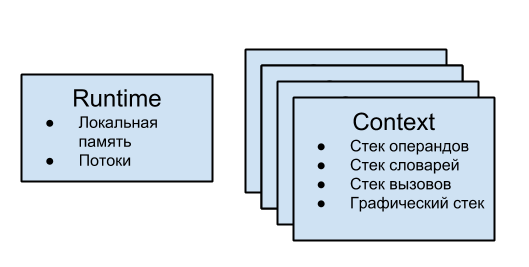
\includegraphics[height=130pt]{Runtime_contexts.png}
		%	\caption{Схема Runtime и контекстов}\label{runtime_contexts}
		%\end{figure}
		
	\begin{figure} [h]
			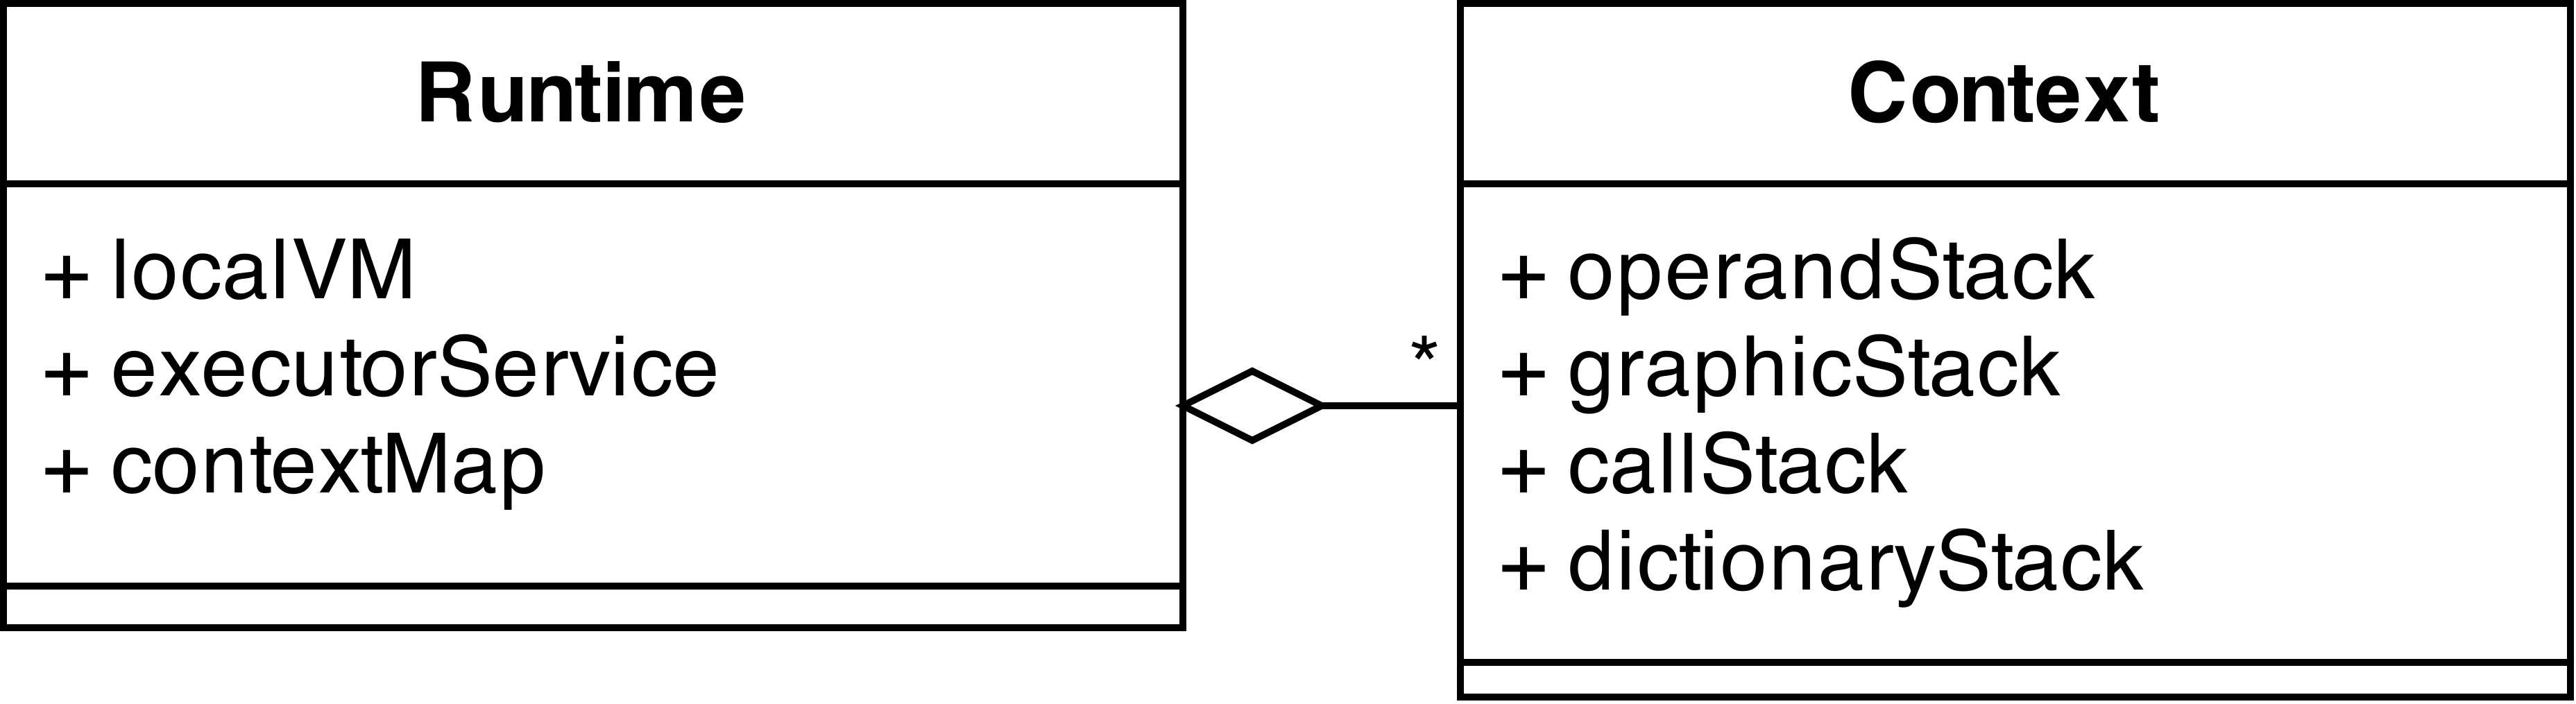
\includegraphics[width=\linewidth]{UML_Runtime_Context.png}
			\caption{Схема Runtime и контекстов}\label{UML_runtime_contexts}
	\end{figure}
		
	\subsection{Библиотека ASM для генерации и изменения байт-кода JVM}
	Библиотека ASM предназначена для создания, изменения и анализа байт-кода Java. Данная библиотека разработана в компании OW2 Consortium~\cite{ow2-site}. Создание классов происходит вызовом соответствующих методов из библиотеки для добавления очередной инструкции JVM. Работа Java Virtual Machine и использование её инструкций подробно описано в спецификации JVM~\cite{jvms}. Этот инструмент очень полезен, если необходимо создавать скомпилированные Java-классы уже после запуска Java-приложения.  Кроме того, собранные классы можно изменять перед загрузкой. Данная функциональность библиотеки активно используется в оптимизации методом динамической компиляции. 


	
	\pagebreak
	\section{Динамическая компиляция процедур}
	%	Динамическая компиляция является одной из реализованных оптимизаций интерпретации программ на языке PostScript. Компиляция происходит только для процедур, но они составляют большую часть программ. 
		%В интерпретаторе JB каждый раз при исполнении процедуры, например, в очередной итерации цикла, эта процедура интерпретируется заново, хотя она не изменилась.
	Для повышения производительности интерпретатора JB были проанализированы узкие места, в которых тратилось большее количество времени. Таковыми оказались процедуры или по-другому исполняемые массивы, которые составляют большую часть программ на PostScript. Они используются в циклах, условных операторах и при их вызове по имени, то есть как вызов функции.  
	В интерпретаторе JB каждый раз при повторном выполнении процедуры происходит повторная интерпретация этой процедуры, например в очередной итерации цикла. На повторную интерпретацию процедур тратится большое количество времени, в то время как его можно уменьшить за счет компиляции процедур.
	Оптимизация интерпретации программ на языке PostScript посредством динамической компиляции процедур исключает проблему повторной интерпретации, динамически компилируя процедуры при их объявлении и после используя скомпилированный байт-код для вызовов процедур.  	
	Эта оптимизация изменила процесс интерпретации: теперь стек вызовов не используется, а вместо процедур создаются «на лету» динамически скомпилированные классы в байт-коде JVM. Далее будет подробно рассмотрена схема создания и использования байт-кода (см. рис. ~\ref{scheme}) и особенности реализации некоторых операторов в данной оптимизации.
	
	%\begin{figure} [h]
	%	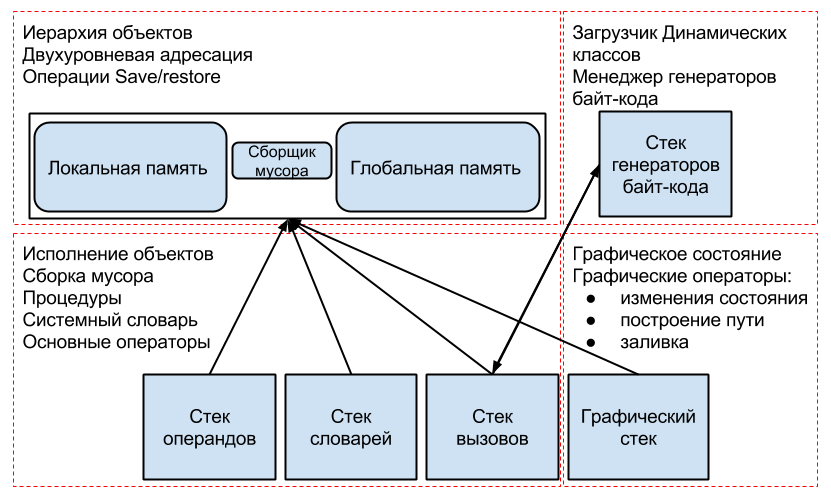
\includegraphics[height=310pt]{Scheme.png}
	%	\caption{Общая схема интерпретатора с оптимизацией}\label{scheme}
	%\end{figure}
	\begin{figure} [h]
		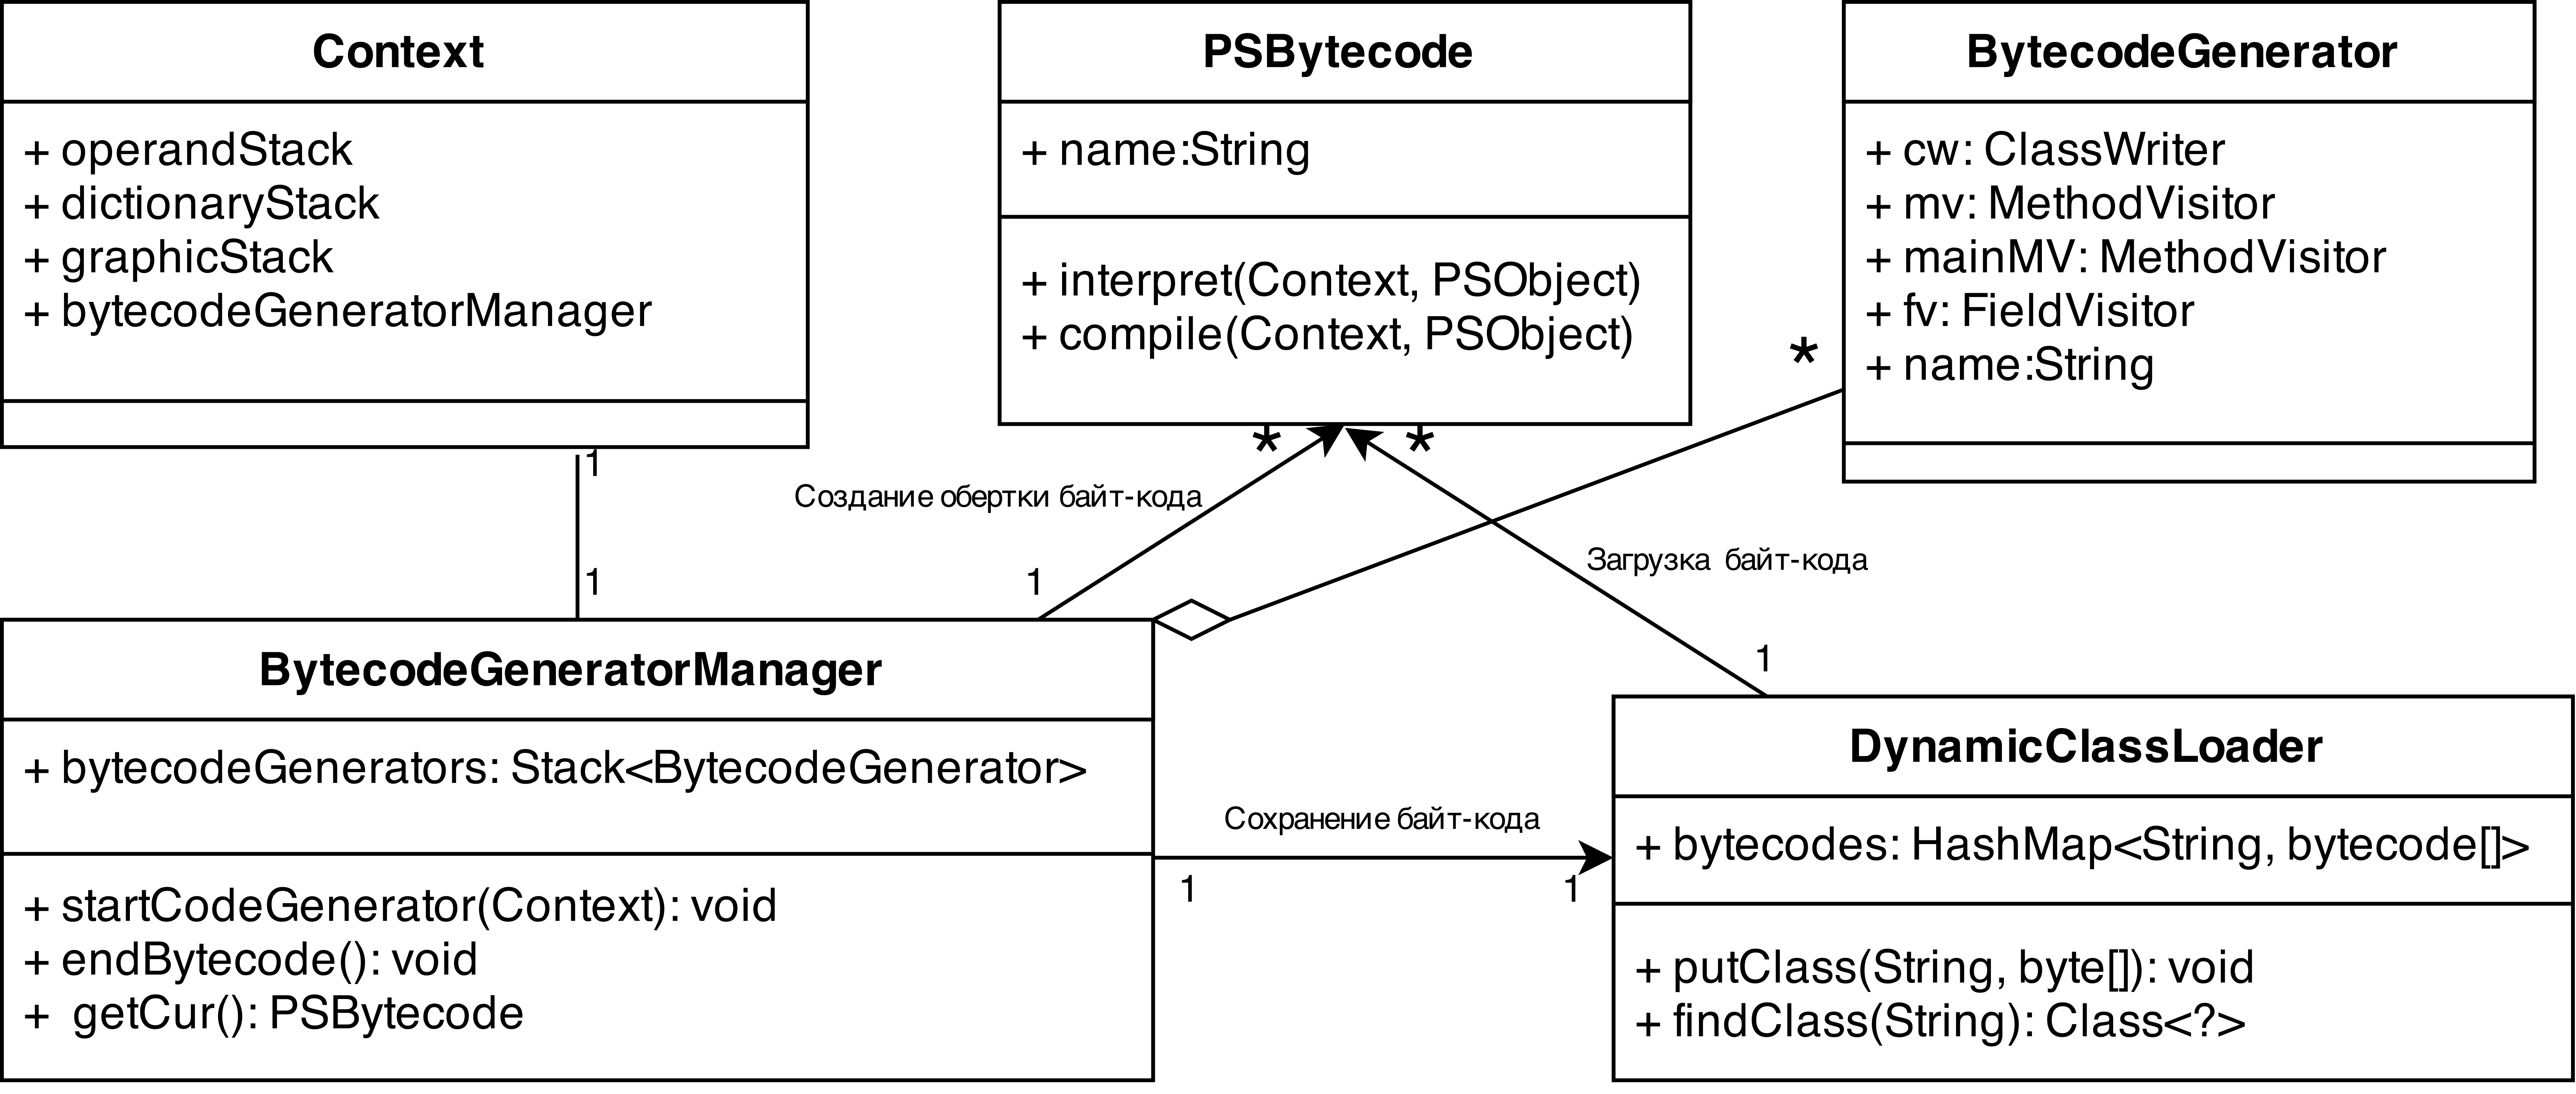
\includegraphics[width=\linewidth]{bytecode_generation.png}
		\caption{Схема классов для создания байт-кода}\label{scheme}
	\end{figure}
	\subsection{Генерация байт-кода}
	\texttt{BytecodeGenerator}  --- главный класс для создания класса в байт-коде для процедуры. Он отвечает за имя класса, наследование, поля, создание конструктора, статическую инициализацию и за объявление начала и конца метода. Содержимое самих методов заполняется инструкциями JVM во время компиляции конкретных объектов. Для добавления инструкций в метод используется соответствующий метод класса \texttt{MethodVisitor} (из библиотеки ASM), например, как в листинге~\ref{PSInteger_compile}. 
	\begin{lstlisting}[label=PSInteger_compile,caption=Компиляция объектов \texttt{Integer} ,captionpos=b, frame = single,language = Java]     mv.visitTypeInsn(NEW, "psObjects/PSObject");
	MethodVisitor mv = context.bcGenManager.mv;
	mv.visitInsn(DUP);
	mv.visitTypeInsn(NEW, "psObjects/values/simple/numbers/PSInteger");
	mv.visitInsn(DUP);
	mv.visitLdcInsn(value);
	mv.visitMethodInsn(INVOKESPECIAL, 
	  "psObjects/values/simple/numbers/PSInteger", "<init>", "(I)V", false);
	mv.visitMethodInsn(INVOKESPECIAL,
	  "psObjects/PSObject", "<init>", "(LpsObjects/values/Value;)V", false);		
	mv.visitFieldInsn(GETSTATIC, name, "context", "Lruntime/Context;");
	mv.visitInsn(ICONST_0);
	mv.visitMethodInsn(INVOKEVIRTUAL,
		"psObjects/PSObject", "interpret", "(Lruntime/Context;I)Z", false);
	\end{lstlisting}
	Для работы с полями класса используется \texttt{FieldVisitor}. Создание класса осуществляется с помощью \texttt{ClassWriter}. После завершения компоновки класса в байт-коде \texttt{BytecodeGenerator}	возвращает массив байтов --- скомпилированный класс.
	
	Процедуры в PostScript могут быть в вложенными, т.е. объявление одной процедуры может быть внутри другой. Компиляция происходит «на лету», т.е. в момент объявления процедуры, из-за этого во время объявления вложенной процедуры создание для внешней ещё не закончено. Поэтому в один и тот же момент времени может быть не закончена интерпретация (а вместе с ней и создание массива) для нескольких процедур.
	
	Для управления процедурами, для которых не завершена компиляция, используется класс \texttt{BytecodeGeneratorManager}. Каждому контексту исполнения (\texttt{Context}) соответствует один менеджер. В нем содержится стек из генераторов байт-кода (\texttt{BytecodeGenerator}), каждый из которых отвечает за свою незавершенную процедуру. На вершине стека находится тот генератор байт-кода, работа с которым идёт в данный момент. Через менеджер можно получить доступ к имени текущего класса и \texttt{MethodVisitor}, в котором определяется текущий метод класса. С помощью менеджера создаются новые генераторы (\texttt{startBytecodeGenerator(Context)}) и завершается создание  байт-кода для процедуры (\texttt{endBytecode()}), после которого происходит сохранение этого байт-кода в \texttt{DynamicClassLoader} с помощью метода \texttt{putClass(String,byte[])}. Каждому имени скомпилированного класса сопоставляется массив байтов (\texttt{bytecodes: HashMap<String,byte[]>}).
	
	Создание байт-кода по процедуре начинается, когда во входном потоке встречается токен "\texttt{\{}"\,, означающий начало исполняемого массива. В этот момент создаётся новый генератор байт-кода и кладется на вершину стека генераторов. После этого для каждого следующего токена в байт-код добавляется несколько инструкций JVM, соответствующих интерпретации данного токена. Для разных типов объектов это происходит по-разному. Когда встречается токен "\texttt{\}}"\,, то завершается создание байт-кода, и его генератор снимается со стека. При этом происходит сохранение скомпилированного класса в виде массива байтов в специальном хранилище, а на стек операндов кладётся объект \texttt{PSBytecode}, в котором хранится только имя скомпилированного класса. 
	\subsubsection*{Исполнение байт-кода}
	Исполнение байт-кода соответствует исполнению процедур в интерпретаторе JB, но реализуется по-другому. В момент вызова байт-код объекта из хранилища скомпилированных классов достаётся массив байтов, соответствующий этому объекту. Затем массив загружается загрузчиком классов (\texttt{ClassLoader}). С этого момента можно уже использовать динамически созданный класс: создавать объекты, вызывать методы и изменять поля у этого класса. Все создаваемые нами классы имеют главный статический метод \texttt{run()}, который выполняет всю работу. Именно этот метод вызывается для выполнения скомпилированной процедуры. После этого происходит исполнение всех инструкций JVM, которые были добавлены в этот класс в момент его генерации.
	
	Во время выполнения байт-кода необходимо использовать внутреннее состояние контекста, а также его изменять (например, брать объект со стека операндов или класть на него). В момент создания байт-кода ещё неизвестно, в каком контексте и потоке он будет вызываться. Это происходит из-за того, что объекты можно передавать между потоками. Поэтому в момент вызова байт-кода передаётся в качестве единственного аргумента текущий контекст, он записывается в качестве поля.
	
	Таким образом, исполнение байт-кода можно разбить на три пункта.
	\begin{itemize}
		\item Загрузка скомпилированного класса загрузчиком классов.
		\item Установление контекста выполнения для загруженного класса.
		\item Вызов статического метода \texttt{run()} у загруженного класса.
	\end{itemize}
	\subsection{Отдельные сложные операторы}
	Из-за изменения схемы интерпретации некоторые стандартные операторы языка, связанные с массивами, реализуются гораздо сложнее, чем первоначально в интерпретаторе JB. 
	\subsubsection*{Оператор связывания \texttt{bind}}
	Данный оператор является системным и заменяет в исполняемом массиве все имена, ссылающиеся на стандартные операторы, на сами операторы.	Во-первых, он предотвращает лишний поиск по словарям. Во-вторых, если после вызова \texttt{bind} переопределится какой-то из операторов, то процедура не изменит хода своего исполнения и будет работать как раньше. Таким образом обеспечивается безопасность в том смысле, что вне зависимости от того, переопределятся ли стандартные операторы или нет, процедура не изменит своего поведения. В примере ~\ref{psExample} перезаписывается оператор \texttt{add}, но это не влияет на работу программы ---  в конце работы программы на стеке лежит число 5. Если бы оператора \texttt{bind} не было в программе, то на вершине стека было бы число 6. Напомним, что оператор \texttt{def} записывает по имени объект, а префикс "/"\,  используется для обозначения литеральных имен.  
		\begin{lstlisting}[float, label=psExample,caption=пример на PostScript на оператор \texttt{bind},captionpos=b, frame = single, language = PostScript]
			/a {2 3 add} bind def
			/add {mul} def
			a
		\end{lstlisting}
	

	Реализация оператора \texttt{bind} осложняется в данной оптимизации тем, что вместо исполняемых массивов используется байт-код, то есть собранный и скомпилированный класс. Причём байт-код нельзя изменять после загрузки в JVM.  Таким образом,  нужно изменять динамически созданный байт-код до загрузки в JVM, что накладывает некоторые ограничения на данную оптимизацию. Оператор \texttt{bind} должен быть вызван до первого вызова процедуры, к которой он относится. Библиотека ASM позволяет модифицировать методы в байт-коде, добавлять и удалять инструкции JVM, то есть инструментировать байт-код. 
	
	Для удобства модификации выделим все «подозрительные» имена в отдельные методы. Здесь «подозрительными» мы назвали те имена, которые ссылаются на системные операторы в момент создания байт-кода. При этом на момент выполнения оператора \texttt{bind} совсем не обязательно, что эти имена всё еще ссылаются на системные операторы. Они могут быть перезаписаны. Именно по этому они «подозрительные».
	
	Поскольку теперь главный метод \texttt{run()} разбит на части, то он выглядел бы следующим образом (см. листинг~\ref{run}), если  бы был он написан на Java. Каждый отдельный метод называется \texttt{run\_<число>}.
	\begin{lstlisting}[label=run,caption=Структура метода run(),captionpos=b, frame = single, language = Java]
	public static void run(){
		run_1();	
		run_2();
		...
		run_m();		
	}
	\end{lstlisting}
	
	В момент компиляции мы запоминаем, какие методы были «подозрительными», то есть содержали вызов «подозрительного»  имени. Запись производится в хеш-таблицу (Hash Map). Ключ --- это пара из номера класса (все классы байт-кода пронумерованы) и номера «подозрительного» метода. А значение, ассоциированное с ключом, является названием того оператора, на который ссылается это подозрительное имя.
	
	Итак, общий алгоритм оператора \texttt{bind} состоит из трёх пунктов:
	\begin{enumerate}
		\item Обнаружение всех «подозрительных» методов в классе с помощью хеш-таблицы.
		\item Выполнение проверки того, перезаписались ли соответствующие им имена. Используются только те, которые всё ещё ссылаются на системные операторы.
		\item Модификация найденных методов:
				\begin{enumerate}
					\item удаление всех инструкций JVM в этих методах кроме последних трёх служебных инструкций;
					\item добавление инструкций, которые вызывают нужный оператор.
				\end{enumerate}				
	\end{enumerate}
	
	После модификации получается уже искомый байт-код, в котором  заменены вызовы имен на операторы.


	\subsubsection*{Оператор  \texttt{cvx}}		
	В языке PostScript системный оператор \texttt{cvx} изменяет атрибут объекта: литеральный делает исполняемым. Поскольку схема интерпретации изменена только для процедур (исполняемых массивов), то с ними возникают некоторые сложности, когда из массива необходимо сделать байт-код. Необходима компиляция массива целиком со всеми объектами. Отличие компиляции на «лету» от компиляции байт-кода по массиву состоит в том, что в первом случае компилируются только отдельные токены, и поэтому компиляция составных объектов, таких как массивы и словари, не происходит.  Они создаются уже на этапе выполнения байт-кода, поскольку состоят из нескольких токенов. Во время компиляции байт-кода по массиву, необходимо компилировать любые входящие в массив объекты, в том числе составные.
	
	Таким образом, для оператора \texttt{cvx} необходимо дополнительно реализовывать  компиляцию сложных объектов, значения которых отделены от объекта и загружены в память, локальную или глобальную. Проблема состоит в том, что в контекст байт-кода можно передавать только неизменяемые объекты и примитивы (с точки зрения Java), которые хранятся в пуле констант Java, а именно: строки и числа. Любые композитные объекты нельзя передавать, т.к. они могут быть изменены.
	
	В случае локальной памяти, где значения сложных объектов хранятся по номеру, данная проблема решается просто. Для восстановления сложного объекта в контексте байт-кода нужно передать его номер в локальной памяти и атрибуты, закодированные с помощью чисел. Так при исполнении байт-кода создаются новые объекты со старыми значениями и атрибутами.
	
	В случае глобальной памяти, где значения хранятся не по номеру в таблице, а по ссылке, решить проблему тем же способом не удаётся. Поэтому самый простой и очевидный способ --- это завести специальную таблицу для сложных объектов, находящихся в глобальной памяти, которые загружаются в байт-код оператором \texttt{cvx}. Из-за того что это довольно редкое событие (оператор \texttt{cvx} нечасто используется, и, в основном, используют локальную память), данное решение не влечет бóльших накладных расходов. В этой таблице по номеру можно найти значение из глобальной памяти, которое нужно загрузить в байт-код.
	
	Таким образом осуществляется компиляция сложных объектов, которая потребовалась в реализации оператора \texttt{cvx}. Простые же операторы компилируются аналогично тому, как это происходит в компиляции на «лету», передавая в байт-код своё примитивное значение.
	\subsubsection*{Оператор выгрузки массива \texttt{aload}}
	Данный оператор в некотором смысле противоположен оператору \texttt{cvx}. Он разгружает массив (при этом не важно, исполняемый или литеральный), т.е кладёт на стек операндов все элементы массива и в конце сам массив. Сложности возникают в случае исполняемого массива, т.е байт-кода в данной оптимизации.
	
	Казалось бы, всё что можно сделать с байт-кодом --- это вызвать его, что значит исполнить все скомпилированные в нем объекты. Но это не то, что требуется в данном операторе. Поэтому реализовано некое «литеральное исполнение» объекта, когда он просто кладётся на стек. Во время вызова любого объекта будем проверять специальный флаг (\texttt{aloading}). Если  в нём записана истина, то вместо исполнения конкретного значения, этот объект сразу кладётся на стек.
	
	Поэтому реализация оператора \texttt{aload} выглядит следующим образом.
	\begin{enumerate}
		\item Установить флаг \texttt{aloading\,=\,true}  в текущем контексте.
		\item Вызвать байт-код.
		\item Положить байт-код на стек операндов.
		\item Установить флаг \texttt{aloading\,=\,false} в текущем контексте.
	\end{enumerate}
	
	Для правильного исполнения оператора \texttt{aload} необходимо, чтобы из байт-кода вызывалось исполнение каждого объекта (т.е. централизованно через один метод). Из-за этого компиляция всех объектов состоит из двух основных частей: «сборка» объекта (внутри него «сборка» его значения) и вызов объекта c помощью метода \texttt{iterpret()} как показано в листинге~\ref{PSInteger_compile} на странице~\pageref{PSInteger_compile}. Там происходит  создание \texttt{PSInteger} по переданному значению, создание объекта \texttt{PSObject} на его основе и вызов интерпретации этого объекта с нужными параметрами. 
	\pagebreak
	\section{Спекулятивная компиляция}
	Объекты-имена встречаются в программах на языке PostScript очень часто, в них записываются либо конкретные неисполняемые значения (в этом случае имена выполняют роль переменных), либо процедуры, исполняемые массивы (здесь имена выполняют роль вызова процедур). Кроме того, в этих двух случаях можно выделить следующие особенности. Имена, ссылающиеся на процедуры, крайне редко перезаписываются, в то же время имена, ссылающиеся на неисполняемые объекты, довольно часто перезаписываются. При этом последних обычно значительно меньше.
	
	Исполнение объекта-имени в интерпретаторе JB происходит следующим образом. Перебираются словари, находящиеся на стеке словарей. Если в текущем словаре есть данное имя и ассоциированное с ним значение, то поиск прекращается, и исполняется найденное значение. При этом словарь является деревом, как структура данных. Получается, что поиск ассоциированного с именем значения --- долгая и дорогостоящая операция. 
	
	В данной оптимизации можно предотвратить повторный поиск по имени при многократном исполнении процедуры, когда  ассоциированное значение уже найдено при определении этой процедуры, и после оно не менялось. В этом и состоит спекулятивная компиляция.
	
	\subsection{Особенности реализации}
	Для этой оптимизации изменён способ компиляции для исполняемых объектов-имён. Сначала происходит поиск ассоциированного с именем значения. Если оно не найдено, то компиляция для этого имени происходит без данной оптимизации, т.е. генерируется код, отвечающий за поиск и вызов значения. Поскольку в PostScript используется стратегия вычислений \texttt{вызов по имени} (англ. "call-by-name"), то значение имени может быть определено позже, чем определение процедуры, использующее это имя.
	
	Если ассоциированное значение найдено, то оно записывается в переменную и используется далее при кэшировании.
	Для проверки актуальности закэшированного значения сравнивается «версии имён» на момент компиляции и на момент исполнения. Во время новых определений для имен и в момент обновления стека словарей сохраняется номер текущей версии для каждого имени. Сравнение версий происходит внутри байт-кода. Если версии имен совпадают, то исполняется закэшированное значение, иначе имя исполняется без оптимизации. Повторного кэширования не происходит, поэтому имена, у которых изменено значение хотя бы один раз при вызове какой-то процедуры (например, счетчик), исполняются в этой процедуре без оптимизации. 

	
	\pagebreak
	\section{Тестирование}
	Во процессе разработки оптимизаций регулярно выполнялось регрессионное тестирование с целью проверки корректности работы основных операторов языка PostScript, используя unit-тесты. Также вместе с разработкой пополнялась база тестов. Каждый из этих тестов содержал короткую программу на PostScript, использовавшая только определенный набор операторов. В результате работы этой программы на стеке операндов появляются конкретные значения. Производилось сравнение состояния стека операндов после работы интерпретатора в двух режимах: с оптимизациями и без них. Поскольку все тесты прошли проверку успешно, то можно сделать вывод, что не смотря на то, что в данных оптимизациях изменен способ интерпретации, семантика выполнения программ осталась неизменна.
	
	Далее была протестирована производительность интерпретатора JB c учетом оптимизаций на значительном наборе тестов-рисунков.	Каждый тест --- это программа на языке PostScript, в результате работы которой на экране показывается изображение. Измерено время работы интерпретатора в трёх режимах: без оптимизаций, с одной оптимизацией (динамическая компиляция) и сразу с двумя оптимизациями (спекулятивная компиляция работает только в вместе с динамической компиляцией). Все тесты можно условно поделить на две большие группы: простые и сложные. Простые --- это тесты, в которых содержится мало трудоёмких операций и время их выполнения не превышает двух секунд с использованием оптимизации (это разделение довольно условное). Остальные --- сложные. Из-за большого количества трудоёмких операций они выполняются значительно дольше.
	
	Сравним быстродействие интерпретатора JB с оптимизациями и без них на компьютерах с системными параметрами, указанными в таблице~\ref{tab:config}.\\



	\begin{table}[h]
		\begin{center}
			\begin{tabular}{|c|c|}
				\hline Процессор & Intel(R) Core(TM) i7-4790 CPU @ 3.60GHz  \\
				\hline Оперативная память & 16 GB \\
				\hline Операционная система & Windows 8 x64 \\
				\hline 
			\end{tabular}
		\end{center}
		\caption{\label{tab:config}Конфигурация компьютера, на котором проводилось тестирование}
	\end{table}
	%\pagebreak
	\subsection*{Простые тесты}
	Результаты тестирования набора простых тестов приведены в табл.~\ref{tab:fast-tests} и на двух графиках на рис.~\ref{graphic: fast}. Между собой тесты не связаны и упорядочены в порядке увеличения времени. На оси абсцисс отмечены номера тестов. Два графика понадобилось для лучшего визуального представления, поскольку диапазон времени исполнения слишком большой: от двух миллисекунд до 4 секунд.
	
	На первом графике, где представлены тесты с наименьшим временем, видно, что интерпретация без оптимизации почти везде работает быстрее, чем с оптимизациями. Это связано с накладными расходами, возникающими при компиляции. На втором графике, на котором представлены тесты с чуть большим временем выполнения, можно заметить, что оптимизации дают выигрыш во времени, но, в основном, незначительный. Из этого можно сделать вывод, что оптимизация интерпретатора на таких простых и коротких программах не требуется.\\
\newcommand{\comma}[0]{,}
		\begin{figure} [h]
			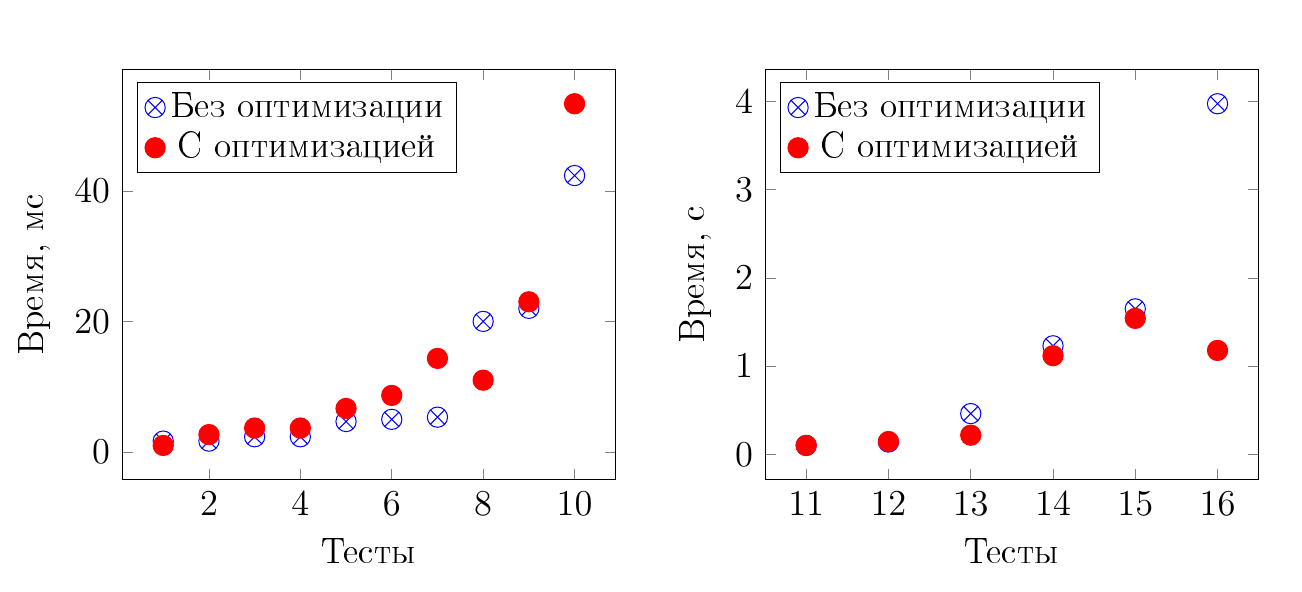
\includegraphics[width=\linewidth]{FastTests.png}
			\caption{Время работы простых тестов}\label{graphic: fast}
		\end{figure}
		\iffalse

\begin{figure}[H]
	\begin{minipage}[h]{0.49\linewidth}
		\center{ 
			\tikzset{every mark/.append style={scale=2}}
			\begin{tikzpicture}
			\begin{axis}[legend pos = north west,ylabel=Время\comma~мс,xlabel=Тесты ]
			\addplot[blue,only marks,mark=otimes] coordinates {
				(1, 1.667   )(2, 1.667   )(3, 2.333   )(4, 2.333   )(5, 4.667   )(6, 5.000   )(7, 5.333   )	(8, 20.000  )(9, 22.000  )(10,42.333  )
			};
			\addlegendentry{Без оптимизации}
			\addplot[red,only marks,mark=*] coordinates {
				(1,    1.000)(2,    2.667)(3,    3.667)(4,    3.667)(5,    6.667)(6,    8.667)(7,    14.333)			(8,   11.000)(9,   23.000)(10,  53.333)	
			};
			\addlegendentry{С оптимизацией}
			\end{axis}
			\end{tikzpicture}
			}
	\end{minipage}
	\hfill
	\begin{minipage}[h]{0.49\linewidth}
		\center{
			\tikzset{every mark/.append style={scale=2}}
			\begin{tikzpicture}
			\begin{axis}[legend pos = north west, ylabel=Время\comma~с, xlabel=Тесты ]
			\addplot[blue,only marks,mark=otimes] coordinates {
					(11,0.100667 )(12,0.139333 )(13,0.462333 )	(14,1.230667)	(15,1.649333)	(16,3.975333)
			};
			\addlegendentry{Без оптимизации}
			\addplot[red,only marks,mark=*] coordinates {
				(11, 0.101000)(12, 0.145333)(13, 0.217000)	(14,1.118333)(15,1.541667)	(16,1.178000)
			};
			\addlegendentry{С оптимизацией}
			\end{axis}
			\end{tikzpicture}}
	\end{minipage}
	\caption{Время работы простых тестов}
	\label{graphic: fast}
\end{figure}
\fi
\begin{table}[H]
	\small
	\begin{center}
	\begin{tabular}{|c|c|c|}
		\hline \textbf{Название теста} & \textbf{Без оптимизации, мс} & \textbf{С оптимизацией, мс}\\
		\hline 7\_ellipses.ps & 1,667 &  2,667\\
		\hline 6\_arcs.ps & 1,667 & 1,000\\
		\hline 1\_rectangles.ps & 2,333 & 3,667\\
		\hline 5\_star.ps &  2,333 & 3,667\\
		\hline flower.ps & 4,667 & 6,667\\
		\hline 2\_trapezoid.ps & 5,000 & 8,667\\
		\hline drop.ps & 5,333 & 14,333\\
		\hline 1\_clip.ps & 20,000 & 11,000\\
		\hline 4\_circles.ps & 22,000 & 23,000\\
		\hline tiger.eps & 42,333 & 53,333\\
		%\hline Butterfly-Vector\_Sample.ps & 89,667 & 120,333\\
		\hline colorcir.ps & 100,667 & 101,000\\
		\hline doretree.ps & 139,333 & 145,333\\
		\hline WireFrame.eps &  462,333 &  217,000\\
		\hline gingerbread.ps & 1649,333 & 1541,667\\
		\hline 6\_Fractal\_Arrow.ps &  1230,667 & 1118,333\\
		\hline chupcko.ps & 3975,333 &  1178,000\\
		\hline 					
	\end{tabular}
	\end{center}
	\caption{\label{tab:fast-tests}Время работы быстрых тестов}
\end{table}

\pagebreak
	\subsection*{Сложные тесты}
	Программы на PostScript, которые входят в набор сложных тестов, работают продолжительное время, поскольку в них используется большое количество математических операций и вычислительно-сложные алгоритмы, например, построение фрактальных рисунков, рендеринг методом трассировки лучей для каждой точки.
	
	Для сложных тестов выполнены замеры времени выполнения интерпретатора в трех режимах: оригинальная интерпретация (без оптимизаций, рассмотренных в данной работе), интерпретация с одной оптимизацией (динамическая компиляция) и интерпретация с двумя оптимизациями (динамическая и спекулятивная компиляция). Отдельно оптимизация посредством спекулятивной компиляции не представлена, поскольку она работает только вместе с динамической компиляцией. Результаты тестирования представлены на  рис.~\ref{graphic: slow} и в табл.~\ref{tab:slow-tests}.
	В таблице указано для каждого из восьми тестов среднее время выполнения и среднее отклонение во всех режимах, в каждом из которых тесты были запущены по 15 раз. На графике указано, в какое количество раз увеличилась скорость работы интерпретатора JB при использовании одной или двух оптимизаций по сравнению с оригинальной интерпретацией. 
	
	Для сложных тестов заметна разница между временем исполнения программ в интерпретаторе в разных режимах. Это происходит из-за того, что в этих тестах в большом количестве повторно используются процедуры. Процедуры в оптимизации посредством динамической компиляции интерпретируются один раз, при этом создается байт-код по процедуре, который исполняется каждый раз при вызове этой процедуры. В то время как в оригинальной интерпретации процедуры интерпретируются каждый раз заново. Спекулятивная компиляция ещё сокращает время работы для большинства тестов.
%	\iffalse	
		\begin{figure} [h]
			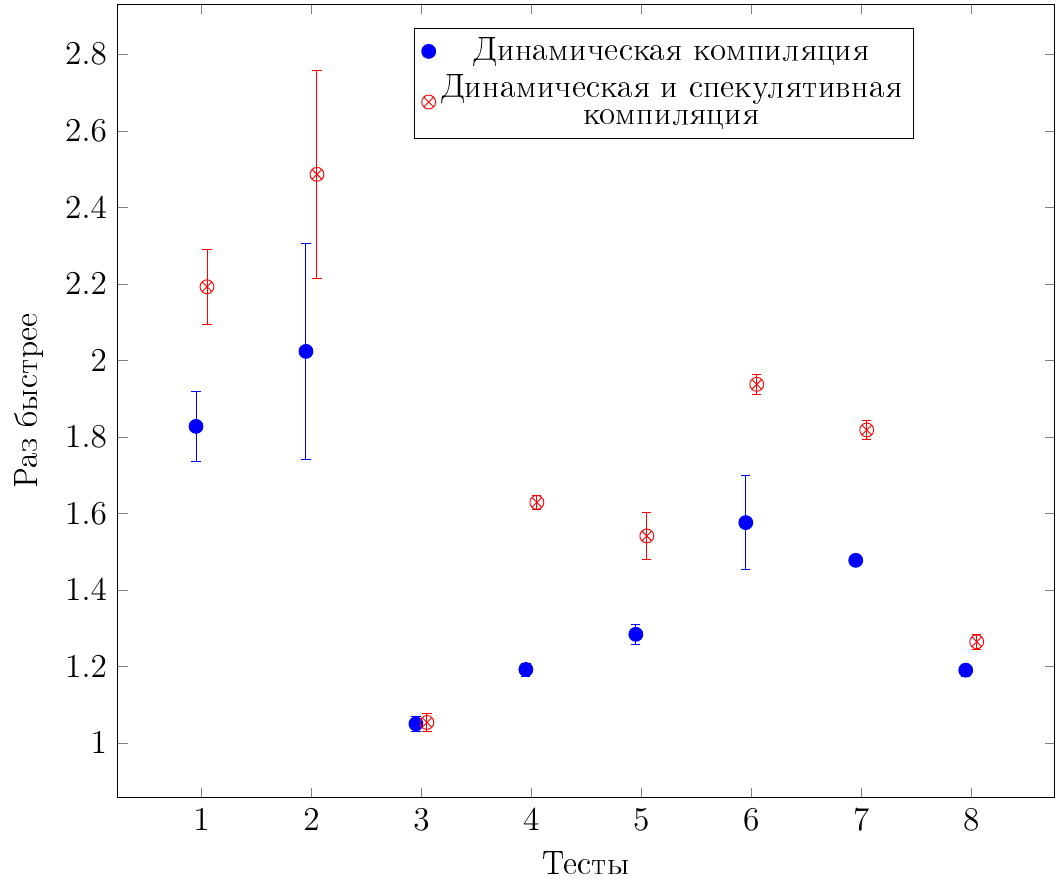
\includegraphics[width=0.87\linewidth]{TimesGraphic.png}
			\caption{Ускорение оптимизаций на сложных тестах}\label{graphic: slow}
		\end{figure}	
	%\fi
		
	\iffalse
	\begin{figure}[H]
			 \tikzset{every mark/.append style={scale=2}}
			 \pgfplotsset{every axis legend/.append style={
			 		at={(1.02,1)},
			 		anchor=north west}}
			 \begin{tikzpicture}
			 \begin{axis}[
			 %legend pos = north west, 
			 ylabel=Время\comma~с,
			 xlabel=Тесты ]                
			 \addplot[blue,only marks,mark=otimes] coordinates {
			(1 ,2.427400  )
			(2 ,10.929000 )
			(3 ,12.622200 )
			(4 ,26.260200 )
			(5 ,60.040400 )
			(6 ,60.001333 )
			(7 ,123.845533)
			(8 ,150.695667)
			(9 ,176.550333)
			(10,323.739133)
			 };
			 \addlegendentry{Оригинальная интерпретация}

			 \addplot[red,only marks,mark=*] coordinates {
			(1 ,1.107400   )
			(2 ,4.396333   )
			(3 ,11.977200  )
			(4 ,16.120400  )
			(5 ,60.041000  )
			(6 ,60.003000  )
			(7 ,80.351400  )
			(8 , 77.780)% пересчитать
			(9 ,97.100400  )
			(10,255.973533 )
			 };
			 \addlegendentry{\shortstack{Динамическая и спекулятивная\\компиляция}}
			 
			 \addplot[black,only marks,mark=square] coordinates {
			 	(1 ,1.328800   )
			 	(2 ,5.401400   )
			 	(3 ,12.017200  )
			 	(4 ,22.025000  )
			 	(5 ,60.050000  )
			 	(6 ,60.003133  )
			 	(7 ,96.43700  )
			 	(8 ,95.612) % пересчитать
			 	(9 ,119.486667 )
			 	(10,271.925000 )
			 };
			 \addlegendentry{Динамическая компиляция}
			 \end{axis}
			 	
			 \end{tikzpicture}
			 \caption{Время работы сложных тестов.}
			 \label{graphic: slow}
	\end{figure}
	\fi
	\iffalse
	\begin{tikzpicture}

		\begin{axis}[	ymode=linear,
		ybar,
		width = 450pt,
		%hight = 350pt,
		/pgf/number format/1000 sep={},
		 ylabel=Время\comma~с,
		 xlabel=Тесты,
		legend style={
			at={(0.67,1.1)},
			%at={(0.5,-0.25)},
%			anchor=south,
			anchor=north east,
			legend columns=1
		}
		]
		\addplot coordinates {
			(1 ,2.427400  )+=(1,0.073) -=(1,0.073)
			(2 ,10.929000 )
			(3 ,12.622200 )
			(4 ,26.260200 )
		%	(5 ,60.040400 )
		%	(6 ,60.001333 )
			(5 ,123.845533)
			(6 ,150.695667)
			(7 ,176.550333)
			(8,323.739133)
		};
		\addplot coordinates {
			(1 ,1.328800   )
			(2 ,5.401400   )
			(3 ,12.017200  )
			(4 ,22.025000  )
			%	(5 ,60.050000  )
			%	(6 ,60.003133  )
			(5 ,96.43700  )
			(6 ,95.612) % пересчитать
			(7 ,119.486667 )
			(8,271.925000 )
		};
		\addplot coordinates {
			(1 ,1.107400   )
			(2 ,4.396333   )
			(3 ,11.977200  )
			(4 ,16.120400  )
		%	(5 ,60.041000  )
		%	(6 ,60.003000  )
			(5 ,80.351400  )
			(6 , 77.780)% пересчитать
			(7 ,97.100400  )
			(8,255.973533 )
			};
		
		\legend{Оригинальная интерпретация, Динамическая компиляция, \shortstack{Динамическая и спекулятивная\\компиляция}}
		\end{axis}
		\end{tikzpicture}
		\fi
		\iffalse
		\begin{tikzpicture}
		
		\begin{axis}[	ymode=linear,
		%ybar,
		width = 450pt,
		%hight = 350pt,
		/pgf/number format/1000 sep={},
		ylabel=\shortstack{Разница во времени между\\ оригинальной интерпретацией и с оптимизациями\comma~с},
		xlabel=Тесты,
		legend style={
			at={(0.75,1.1)},
			%at={(0.5,-0.25)},
			%			anchor=south,
			anchor=north east,
			legend columns=1
		}
		]
		\addplot [
		smooth,
		mark=*,
		blue,
		only marks,
		error bars/.cd, y dir=both, y explicit,
		] plot coordinates {
			(0.95 ,1.099000  )+=(0.95,0.155146) -=(0.95,0.155146)
			(1.95 ,5.528000  )+=(1.95,2.236067) -=(1.95,2.236067)
			(2.95 ,0.605000  )+=(2.95,0.232558) -=(2.95,0.232558)
			(3.95 ,4.235000  )+=(3.95,0.391365) -=(3.95,0.391365)
			(4.95 ,27.408000  )+=(4.95,3.055522) -=(4.95,3.055522)
			(5.95 ,55.083000  )+=(5.95,11.940079) -=(5.95,11.940079)
			(6.95 ,57.064000  )+=(6.95,1.070016) -=(6.95,1.070016)
			(7.95 ,51.814000  )+=(7.95,4.661684) -=(7.95,4.661684)
		};
		\addplot [
		smooth,
		mark=otimes,
		red,
		only marks,
		error bars/.cd,
		y dir=both,
		y explicit,
		] coordinates {
			(1.05 ,1.320000  )+=(1.05,0.148086) -=(1.05,0.148086)
			(2.05 ,6.533000  )+=(2.05,2.031936) -=(2.05,2.031936)
			(3.05 ,0.645000  )+=(3.05,0.291963) -=(3.05,0.291963)
			(4.05 ,10.140000  )+=(4.05,0.330720) -=(4.05,0.330720)
			(5.05 ,43.494000  )+=(5.05,5.851642) -=(5.05,5.851642)
			(6.05 ,72.915000  )+=(6.05,2.386855) -=(6.05,2.386855)
			(7.05 ,79.450000  )+=(7.05,2.586400) -=(7.05,2.586400)
			(8.05 ,67.766000  )+=(8.05,5.270083) -=(8.05,5.270083)
		};

		
		\legend{Динамическая компиляция - оригинальная , \shortstack{Динамическая и спекулятивная\\компиляция - оригинальная} }
		\end{axis}
		\end{tikzpicture}
		\fi
		\iffalse
		\begin{figure} [h]	
				\begin{tikzpicture}
				\tikzset{every mark/.append style={scale=1.5}}
				\begin{axis}[	ymode=linear,
				%ybar,
				width = 450pt,
				%hight = 350pt,
				/pgf/number format/1000 sep={},
				ylabel=Раз быстрее,
				xlabel=Тесты,
				legend style={
					at={(0.85,0.97)},
					%at={(0.5,-0.25)},
					%			anchor=south,
					anchor=north east,
					legend columns=1
				}
				]
				\addplot [
				smooth,
				mark=*,
				blue,
				only marks,
				error bars/.cd, y dir=both, y explicit,
				] plot coordinates {
					(0.95 ,1.827560  )+=(0.95,0.092000) -=(0.95,0.092000)
					(1.95 ,2.023514  )+=(1.95,0.283000) -=(1.95,0.283000)
					(2.95 ,1.050345  )+=(2.95,0.019000) -=(2.95,0.019000)
					(3.95 ,1.192281  )+=(3.95,0.017000) -=(3.95,0.017000)
					(4.95 ,1.284206  )+=(4.95,0.026000) -=(4.95,0.026000)
					(5.95 ,1.576110  )+=(5.95,0.122000) -=(5.95,0.122000)
					(6.95 ,1.477579  )+=(6.95,0.008000) -=(6.95,0.008000)
					(7.95 ,1.190545  )+=(7.95,0.016000) -=(7.95,0.016000)
				};
				\addplot [
				smooth,
				mark=otimes,
				red,
				only marks,
				error bars/.cd,
				y dir=both,
				y explicit,
				] coordinates {
					(1.05 ,2.192412  )+=(1.05,0.098000) -=(1.05,0.098000)
					(2.05 ,2.486124  )+=(2.05,0.272000) -=(2.05,0.272000)
					(3.05 ,1.053853  )+=(3.05,0.024000) -=(3.05,0.024000)
					(4.05 ,1.629032  )+=(4.05,0.018000) -=(4.05,0.018000)
					(5.05 ,1.541300  )+=(5.05,0.062000) -=(5.05,0.062000)
					(6.05 ,1.937452  )+=(6.05,0.026000) -=(6.05,0.026000)
					(7.05 ,1.818229  )+=(7.05,0.025000) -=(7.05,0.025000)
					(8.05 ,1.264739  )+=(8.05,0.019000) -=(8.05,0.019000)
				};
				
				
				\legend{Динамическая компиляция , \shortstack{Динамическая и спекулятивная\\компиляция} }
				\end{axis}
				\end{tikzpicture}
				\caption{Ускорение оптимизаций на сложных тестах}
				\label{graphic: slow}
		\end{figure}
	\fi
	\iffalse	
	\begin{table}[H]
		\small
		\begin{center}
			\begin{tabular}{|c|c|c|c|}
				\hline 	\textbf{\shortstack{Название\\теста}} & \textbf{\shortstack{Оригинальная\\ интерпретация, с}} & \textbf{\shortstack{Динамическая\\компиляция, с}} & \textbf{\shortstack{Динамическая\\ и спекулятивная\\компиляция, с}}\\
			  \hline chupcko.ps&2.427 (3.0\%) &1.328 (6.2\%)&1.107 (6.8\%)\\
			  \hline bubbles.ps&10.929 (12.8\%) &5.401 (15.5\%)&4.396 (14.4\%)\\
			  \hline henon.ps&12.622 (0.7\%) &12.017 (1.2\%)&11.977 (1.7\%)\\
			  \hline mandelbrotset.ps&26.260 (0.4\%) &22.025 (1.3\%)&16.120 (1.4\%)\\
			  \hline AlunJones.ps&60.040 (0.0\%) &60.050 (0.0\%)&60.041 (0.0\%)\\
			  \hline AlunJones2.ps&60.001 (0.0\%) &60.003 (0.0\%)&60.003 (0.0\%)\\
			  \hline julia.ps&123.845 (2.0\%) &96.437 (0.6\%)&80.351 (4.2\%)\\
			  \hline psRay.ps&150.695 (0.5\%) &95.612 (11.7\%)&77.780 (2.1\%)\\
			  \hline mandel.ps&176.550 (0.2\%) &119.486 (0.6\%)&97.100 (2.3\%)\\
			  \hline 1dca.ps&323.739 (0.6\%) &271.925 (1.0\%)&255.973 (1.3\%)\\
		  	  \hline 	
			\end{tabular}
		\end{center}
		\caption{\label{tab:slow-tests}Время работы сложных тестов}
	\end{table}
	
	
	\fi	
	
		\begin{table}[H]
			\small
			\begin{center}
				\begin{tabular}{|c|c|c|c|c|}
					\hline \textbf{Номер} &	\textbf{\shortstack{Название\\теста}} & \textbf{\shortstack{Оригинальная\\ интерпретация, с}} & \textbf{\shortstack{Динамическая\\компиляция, с}} & \textbf{\shortstack{\\Динамическая\\ и спекулятивная\\компиляция, с}}\\
					\hline 1&chupcko.ps&2.427 $\pm$ 0.073&1.328 $\pm$ 0.082&1.107 $\pm$ 0.075\\
					\hline 2&bubbles.ps&10.929 $\pm$ 1.399&5.401 $\pm$ 0.837&4.396 $\pm$ 0.633\\
					\hline 3&henon.ps&12.622 $\pm$ 0.088&12.017 $\pm$ 0.144&11.977 $\pm$ 0.204\\
					\hline 4&mandelbrotset.ps&26.260 $\pm$ 0.105&22.025 $\pm$ 0.286&16.120 $\pm$ 0.226\\
					\hline 5&julia.ps&123.845 $\pm$ 2.477&96.437 $\pm$ 0.579&80.351 $\pm$ 3.375\\
					\hline 6&psRay.ps&150.695 $\pm$ 0.753&95.612 $\pm$ 11.187&77.780 $\pm$ 1.633\\
					\hline 7&mandel.ps&176.550 $\pm$ 0.353&119.486 $\pm$ 0.717&97.100 $\pm$ 2.233\\
					\hline 8&1dca.ps&323.739 $\pm$ 1.942&271.925 $\pm$ 2.719&255.973 $\pm$ 3.328\\
					\hline 	
				\end{tabular}
			\end{center}
			\label{tab:slow-tests}
			\caption{Время работы сложных тестов}
		\end{table}
	По результатам тестирования сложных тестов можно сделать вывод, что рассмотренные в данной работе оптимизации позволяют получить выигрыш во времени до двух раз на некоторых сложных, затратных задачах.
	\pagebreak
	\section*{Заключение}
	\addcontentsline{toc}{section}{Заключение}
	
	В рамках дипломной работы получены следующие результаты.
	\begin{itemize}
		\item Выполнена оптимизация исполнения программ на языке PostScript в среде JVM посредством динамической компиляции (JIT).
		\begin{itemize}
			\item Проведена динамическая компиляция процедур «на лету» (при их инициализации) способом генерации байт-кода JVM (библиотека ASM).
			\item Осуществлена замена стека исполнения стеком генераторов байт-кода.
		\end{itemize}
		\item Выполнена оптимизация исполнения программ на языке PostScript в среде JVM посредством спекулятивной компиляции.
		\begin{itemize}
			\item Компиляция проводится при предположении, что значения большинство имен, ссылающихся на процедуры, не меняются.
			\item Производится кэширование имен при компиляции, если по имени записано значение.
		\end{itemize}
		\item  Выполнены эксперименты по замеру производительности, показавшие увеличение быстродействия в два раза по сравнению со стандартной реализацией. 
	\end{itemize}
	
	\pagebreak
	\bibliographystyle{ugost2008ls}
	
	\addcontentsline{toc}{section}{Список литературы}
	\begin{thebibliography}{99}
		\bibitem{GS-site}
		Официальная страница интерпретатора GhostScript. \\
		\url{http://www.ghostscript.com/}
		
		\bibitem{Adobe-PS-site}
		Официальная страница интерпретатора Adobe PostScript. \\
		\url{http://www.adobe.com/products/postscript/}
		
		\bibitem{PLRM}
		Спецификация языка Postscript. PostScript Language reference. \\
		Adobe Systems. 1999\\
		\url{http://www.adobe.com/products/postscript/pdfs/PLRM.pdf}
		
		\bibitem{artifex-site}
		Официальная страница компании Artifex Software. \\
		\url{	http://www.artifex.com/}

		\bibitem{runtime}
		Дмитрий Поздин. Реализация общей поддержки времени исполнения для интерпретатора языка PostScript.// Труды лаборатории языковых инструментов. Выпуск 2. 2014. с. 276-296.
		
		\bibitem{graphic}
		Артур Гудиев.
		Реализация графической части интерпретатора языка PostScript.// Труды лаборатории языковых инструментов. Выпуск 2. 2014. с. 297-312.

		\bibitem{architecture}
		Рустам Макулов.
		Архитектура интерпретатора для исполнения программ на языке PostScript в JVM. // Труды лаборатории языковых инструментов. Выпуск 2. 2014. с. 259-275.
		
		
		\bibitem{patterns}
		Эрих Гамма, Ричард Хелм, Ральф Джонсон, Джон Влиссидс. \\ Приёмы объектно-ориентированного проектирования. Паттерны проектирования.  1994

		\bibitem{ow2-site}
		Официальная страница компании OW2 Consortium. \\
		\url{www.ow2.org/}
				
		\bibitem{jvms}
		Tim Lindholm, Frank Yellin, Gilad Bracha, Alex Buckley.
		The Java Virtual Machine Specification.
		Java SE 7 Edition, 2013. \\
		\url{docs.oracle.com/javase/specs/jvms/se7/jvms7.pdf}
		



				

		
	\end{thebibliography}
	\pagebreak
	
	
\end{document}
